\documentclass[11pt]{article}

% ── Layout ──────────────────────────────────────────────────────────
\usepackage[margin=1in,top=1in,bottom=1in]{geometry}

% ── Typography ──────────────────────────────────────────────────────
\usepackage[T1]{fontenc}
\usepackage{lmodern}               % Latin Modern text + math
\usepackage[scaled=0.88]{helvet}   % Helvetica for sans-serif
\usepackage{courier}               % Courier for mono
\usepackage{microtype}             % Optical adjustments
\linespread{1.08}                  % Slight spread for readability

% ── Packages ────────────────────────────────────────────────────────
\usepackage{graphicx}
\usepackage{booktabs}
\usepackage{enumitem}
\usepackage{caption}
\usepackage{float}
\usepackage{needspace}
\usepackage[table]{xcolor}
\usepackage{titlesec}
\usepackage{fancyhdr}
\usepackage{tcolorbox}
\usepackage{tikz}
\usetikzlibrary{arrows.meta,positioning,shapes.geometric,fit,backgrounds,calc}
\usepackage[colorlinks,linkcolor=NavyBlue,citecolor=NavyBlue,urlcolor=NavyBlue]{hyperref}

% ── Colors ──────────────────────────────────────────────────────────
\definecolor{NavyBlue}{RGB}{0,51,102}
\definecolor{LightGray}{RGB}{245,245,245}
\definecolor{MedGray}{RGB}{128,128,128}
\definecolor{TableShade}{RGB}{248,248,252}

% ── Section formatting ──────────────────────────────────────────────
\setlength{\parskip}{4pt plus 1pt}
\setlength{\parindent}{0pt}
\setlist{nosep,leftmargin=*}

\titlespacing*{\section}{0pt}{10pt}{4pt}
\titlespacing*{\subsection}{0pt}{8pt}{2pt}
\titleformat{\section}{\normalfont\bfseries\normalsize\scshape}{\thesection}{0.6em}{}
\titleformat{\subsection}{\normalfont\bfseries\small}{\thesubsection}{0.5em}{}

% ── Captions ────────────────────────────────────────────────────────
\setlength{\abovecaptionskip}{6pt}
\setlength{\belowcaptionskip}{2pt}
\captionsetup{font=small,labelfont={bf,small},labelsep=period,format=hang}

% ── Table row spacing ──────────────────────────────────────────────
\renewcommand{\arraystretch}{1.15}

% ── Headers/footers ────────────────────────────────────────────────
\pagestyle{fancy}
\fancyhf{}
\renewcommand{\headrulewidth}{0pt}
\fancyfoot[C]{\small\thepage}

% ── Prompt boxes ───────────────────────────────────────────────────
\tcbset{
  promptbox/.style={
    colback=LightGray,
    colframe=LightGray,
    boxrule=0pt,
    arc=2pt,
    left=8pt,right=8pt,top=6pt,bottom=6pt,
    fontupper=\small\ttfamily,
  }
}

% ── Prevent large vertical gaps ───────────────────────────────────
\raggedbottom

% ═══════════════════════════════════════════════════════════════════
\begin{document}

% ── Title block ────────────────────────────────────────────────────
\begin{center}
\vspace{4pt}
{\LARGE\bfseries Autoreason: Self-Refinement That Knows When to Stop}\\[10pt]
{\normalsize SHL0MS \enspace$|$\enspace HERMES AGENT}\\[2pt]
{\small\textcolor{MedGray}{\href{https://github.com/NousResearch/autoreason}{github.com/NousResearch/autoreason}}}\\[12pt]
\end{center}

% ── Abstract ───────────────────────────────────────────────────────
\noindent\textbf{\scshape Abstract.}\enspace
Iterative self-refinement fails for three reasons: \textit{prompt bias}, where adversarial critique prompts cause models to hallucinate problems that don't exist; \textit{scope creep}, where each revision pass expands the document's scope unchecked; and \textit{lack of restraint}: models almost never decline to make changes, even when the output is already good. Together these guarantee progressive degradation. We present autoreason, which addresses all three by structuring each iteration as a three-way choice: the unchanged incumbent~(A), an adversarial revision~(B), and a synthesis~(AB). Fresh agents with no prompt history or session context judge the candidates via blind Borda count, ensuring that ``do nothing'' is always a first-class option, and the evaluators share none of the biases that produced the revisions. The method's value is greatest at mid-tier models, where the gap between generation capability and self-evaluation capability is widest. With Haiku~3.5 (${\sim}$10$\times$ cheaper than Sonnet~4), autoreason scored 42/42 Borda across three tasks, a perfect sweep, while standard refinement baselines \textit{degraded} the same model's outputs below its unrefined single pass. Across five model tiers (Llama~8B, Gemini~Flash, Haiku~3.5, Haiku~4.5, Sonnet~4), the advantage peaks at mid-tier and diminishes at both extremes: models too weak to generate diverse alternatives (Llama) or too strong to need external evaluation (Sonnet~4.6). Haiku~4.5 confirms the transition: at 60\% private-test accuracy on code (matching Sonnet single-pass), autoreason's gains on held-out tests vanish entirely, despite a 4pp lift on visible tests.

We validate across 5~subjective writing tasks, 150~competitive programming problems (CodeContests) at four model tiers, a five-tier model capability comparison, and systematic ablations of judge count, aggregation method, component necessity, and length bias. In code, autoreason achieves 77\% private-test accuracy vs.\ 73\% for single-pass with Sonnet~4.6. With weaker Haiku~3.5 authors, autoreason outperforms best-of-6 sampling (40\% vs.\ 31\%) at matched compute, while critique-and-revise degrades below single-pass. With stronger Haiku~4.5 authors, the advantage disappears on held-out tests (60\% for all strategies), confirming the method's value is bounded by the generation-evaluation gap. Length-controlled evaluation confirms gains survive when outputs are truncated to matched word counts. The practical recommendation: autoreason operates in the space where models can generate diverse alternatives but cannot reliably choose between them.

\vspace{10pt}
\hrule
\vspace{12pt}

\section{Introduction}

Iterative LLM self-refinement is widely assumed to improve outputs, but the evidence is mixed. The failure modes are structural, not incidental. First, \textit{prompt bias}: a critique prompt like ``find problems with this document'' will almost always produce criticism, even when the document is good. The model hallucinates flaws to satisfy the instruction, a form of sycophantic behavior where the model prioritizes adherence to the prompt over accurate assessment~\cite{sycophancy_survey,sycophancy_pinpoint}. Second, \textit{scope creep}: each revision pass adds detail, restructures, and expands, because both models and judges exhibit systematic verbosity bias; longer outputs are preferred regardless of quality~\cite{length_bias,verbosity_bias}. Third, \textit{lack of restraint}: models rarely decline to make changes, even when told to be conservative. The instruction to revise overrides any hedging, and self-correction without external feedback is largely ineffective~\cite{huang2023,selfcorrect_decompose}. Self-Refine~\cite{selfrefine} demonstrates that critique-and-revise loops can help but provides no mechanism to detect when revisions make things worse. SlopCodeBench~\cite{slopcodebench} documents progressive degradation in iterative code generation, and Shukla et al.~\cite{security_degrade} show the same pattern for security properties in iterative code refinement. The question is not whether self-refinement can work, but \textit{when} it works and what makes it fail.

We present autoreason, extending Karpathy's autoresearch~\cite{autoresearch} beyond objective metrics to domains where quality is subjective or multi-dimensional. The key insight is that ``do nothing'' must be a first-class option. Each iteration produces three competing versions: the unchanged incumbent~(A), an adversarial revision~(B), and a synthesis~(AB), evaluated by a blind panel of fresh agents that share none of the prompt biases or session context that produced the candidates. The method constructs a fitness function through the evaluation process itself, and the incumbent survives by default if the alternatives aren't genuinely better. Component ablations confirm that both the adversarial revision and the synthesis are necessary: removing either collapses the tournament, and the incumbent wins immediately without meaningful competition. Length-controlled evaluation confirms the quality gains are not a verbosity artifact.

Our central finding is that \textbf{the value of structured refinement depends on the gap between a model's generation capability and its self-evaluation capability}. Self-refinement fails because evaluation is harder than generation~\cite{huang2023}. Autoreason bridges this gap with external evaluation. Across five model tiers, the advantage peaks at mid-tier models where the gap is widest: Haiku~3.5 achieved a perfect 42/42 Borda while standard baselines \textit{degraded} its outputs below the unrefined starting point (Section~\ref{sec:small}). At the bottom (Llama~8B), the model is too weak to generate diverse alternatives for the tournament. At the top (Sonnet~4.6), the gap is narrow enough that simple methods suffice (Section~\ref{sec:scaling}). Haiku~4.5 marks the transition: strong enough that autoreason's private-test gains vanish on code, despite visible-test improvements (Section~\ref{sec:code}). The method operates in the practical middle, the range where most cost-conscious LLM deployment lives, and where the generation-evaluation gap is large enough to exploit.

Our experiments identify four conditions for the method to succeed: (1)~\textbf{external verification}: providing evaluation capability the generating model lacks; (2)~\textbf{constrained scope}: bounded improvement space; (3)~\textbf{structured reasoning}: explicit failure analysis rather than reactive editing; and (4)~\textbf{sufficient decision space}: the task admits genuinely different valid approaches. We test across subjective writing (5~open-ended tasks, 3~constrained tasks, 8~remedy experiments), competitive programming (150~CodeContests problems across four model tiers), a five-tier model capability comparison (Llama~8B through Sonnet~4.6), and systematic ablations of the method's components (judge count, aggregation, synthesis vs.\ revision, length bias). These conditions are consistent with our results but should be treated as hypotheses supported by evidence, not established laws.

\section{Method}

\begin{figure}[!ht]
\centering
\resizebox{0.95\textwidth}{!}{%
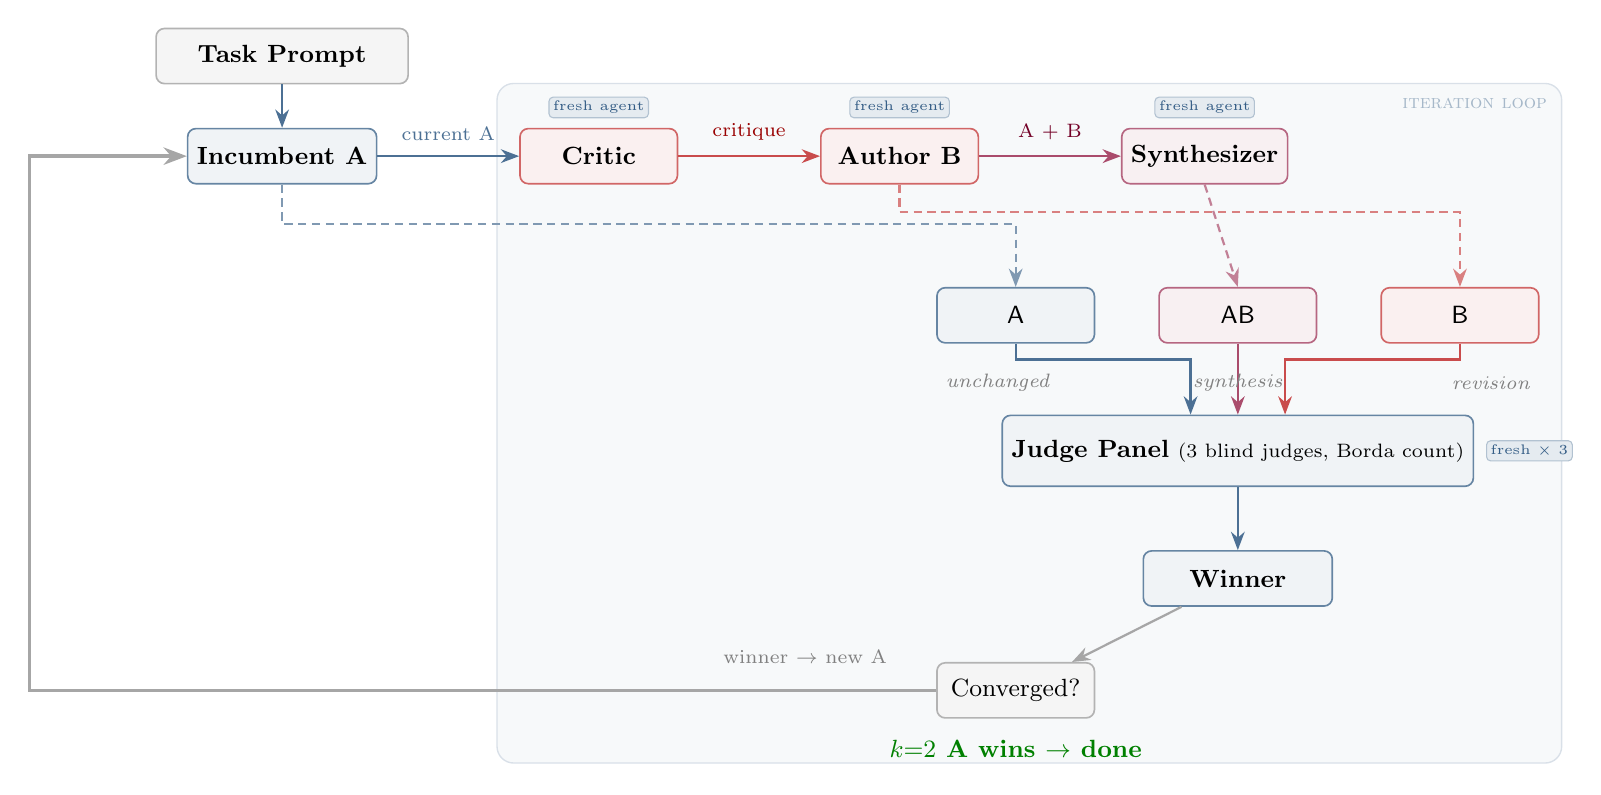
\begin{tikzpicture}[
    >=Stealth,
    node distance=0.6cm and 1.2cm,
    box/.style={rectangle, rounded corners=3pt, draw=#1!60, fill=#1!6,
                minimum height=0.7cm, minimum width=2.0cm,
                font=\small, text=black, line width=0.6pt},
    box/.default=NavyBlue,
    arr/.style={->, thick, color=#1!70},
    arr/.default=NavyBlue,
    dasharr/.style={->, densely dashed, thick, color=#1!50},
    dasharr/.default=NavyBlue,
]

% ── Task prompt anchor ──
\node[box=MedGray, minimum width=3.2cm, fill=LightGray, draw=MedGray!60]
    (task) {\textbf{Task Prompt}};

% ── Incumbent A ──
\node[box, below=0.55cm of task] (A) {\textbf{Incumbent A}};

% ── Critic ──
\node[box=red!70!black, right=1.8cm of A] (critic) {\textbf{Critic}};

% ── Author B ──
\node[box=red!70!black, right=1.8cm of critic] (authorB) {\textbf{Author B}};

% ── Synthesizer ──
\node[box=purple!70!black, right=1.8cm of authorB] (synth) {\textbf{Synthesizer}};

% ── Three candidates: A, AB, B order ──
\node[box, below=1.3cm of synth, xshift=-2.4cm] (candA) {\textsf{A}};
\node[box=purple!70!black, right=0.8cm of candA] (candAB) {\textsf{AB}};
\node[box=red!70!black, right=0.8cm of candAB] (candB) {\textsf{B}};

% ── Judge panel ──
\node[box=NavyBlue, below=0.9cm of candAB, minimum width=4.8cm, minimum height=0.9cm]
    (judge) {\textbf{Judge Panel} {\scriptsize (3 blind judges, Borda count)}};

% ── Winner decision ──
\node[box=NavyBlue, below=0.8cm of judge, minimum width=2.4cm] (winner) {\textbf{Winner}};

% ── Convergence check ──
\node[box=MedGray, fill=LightGray, draw=MedGray!60, below left=0.7cm and 0.6cm of winner,
      minimum width=2.0cm] (conv) {Converged?};

% ── Arrows: main pipeline (top row) ──
\draw[arr] (task) -- (A);
\draw[arr] (A) -- (critic);
\draw[arr=red!70!black] (critic) -- (authorB);
\draw[arr=purple!70!black] (authorB) -- (synth);

% ── Edge labels on pipeline arrows ──
\node[font=\scriptsize, text=NavyBlue!70, above=0.08cm] at ($(A.east)!0.5!(critic.west)$) {current A};
\node[font=\scriptsize, text=red!60!black, above=0.08cm] at ($(critic.east)!0.5!(authorB.west)$) {critique};
\node[font=\scriptsize, text=purple!60!black, above=0.08cm] at ($(authorB.east)!0.5!(synth.west)$) {A + B};

% ── Arrows: candidates down (dashed) ──
\draw[dasharr] (A.south) -- ++(0,-0.5) -| (candA.north);
\draw[dasharr=purple!70!black] (synth.south) -- (candAB.north);
\draw[dasharr=red!70!black] (authorB.south) -- ++(0,-0.35) -| (candB.north);

% ── Arrows: candidates to judge ──
\draw[arr] (candA.south) -- ++(0,-0.2) -| ([xshift=-0.6cm]judge.north);
\draw[arr=purple!70!black] (candAB.south) -- (judge.north);
\draw[arr=red!70!black] (candB.south) -- ++(0,-0.2) -| ([xshift=0.6cm]judge.north);

% ── Judge to winner ──
\draw[arr] (judge) -- (winner);

% ── Winner to convergence check ──
\draw[arr=MedGray] (winner) -- (conv);

% ── Loop back arrow: route along far left, clear of all elements ──
\coordinate (loopleft) at ([xshift=-2.0cm]A.west);
\draw[arr=MedGray, line width=1.2pt]
    (conv.west) -| (loopleft) -- (A.west);
\node[font=\scriptsize, text=MedGray, anchor=south east]
    at ([xshift=-0.5cm, yshift=-0.15cm]conv.north west) {winner $\to$ new A};

% ── Convergence exit ──
\node[font=\small\bfseries, text=green!50!black, below=0.15cm of conv] {$k{=}2$ A wins $\to$ \textrm{done}};

% ── Fresh agent badges: positioned clearly above each role ──
\begin{scope}[every node/.style={font=\tiny, rounded corners=1.5pt,
    fill=NavyBlue!10, draw=NavyBlue!30, inner sep=1.5pt, text=NavyBlue!80}]
    \node[above=0.12cm of critic] {fresh agent};
    \node[above=0.12cm of authorB] {fresh agent};
    \node[above=0.12cm of synth] {fresh agent};
    \node[right=0.15cm of judge.east, anchor=west] {fresh $\times$ 3};
\end{scope}

% ── Role descriptions: positioned below candidates, clear of arrows ──
\node[font=\scriptsize\itshape, text=MedGray, anchor=west]
    at ([yshift=-0.50cm]candA.south west) {unchanged};
\node[font=\scriptsize\itshape, text=MedGray, anchor=center]
    at ([yshift=-0.50cm]candAB.south) {synthesis};
\node[font=\scriptsize\itshape, text=MedGray, anchor=east]
    at ([yshift=-0.50cm]candB.south east) {revision};

% ── Loop region background ──
\begin{scope}[on background layer]
\node[fit=(critic)(candA)(candB)(judge)(winner)(conv),
      rounded corners=6pt, fill=NavyBlue!3, draw=NavyBlue!15,
      inner xsep=8pt, inner ysep=16pt, line width=0.5pt] (loopbg) {};
\node[font=\scriptsize\scshape, text=NavyBlue!35,
      anchor=north east] at ([xshift=-2pt, yshift=-2pt]loopbg.north east) {iteration loop};
\end{scope}

\end{tikzpicture}%
}% end resizebox
\caption{The autoreason loop. Each pass produces three candidates: the unchanged incumbent~(A), a synthesis~(AB), and an adversarial revision~(B). A blind judge panel selects the winner via Borda count. If A survives $k{=}2$ consecutive passes, the loop terminates. Every role is a fresh, isolated agent.}
\label{fig:method}
\end{figure}

\textbf{Critic.}\enspace A fresh agent identifies problems in the current incumbent~A. Finds problems only; no fixes. Optionally receives ground-truth data for fact-checking (Section~\ref{sec:paper}).

\textbf{Author~B.}\enspace A fresh agent revises A based on the critique. Sees the task, A, and the critique. No drafting history.

\textbf{Synthesizer.}\enspace A fresh agent receives A and B with randomized labels. Produces AB by taking the strongest elements of each.

\textbf{Judge Panel.}\enspace 3 fresh agents rank A, AB, B via Borda count (3/2/1 points). Randomized labels and presentation order. Conservative tiebreak: incumbent wins ties. Convergence at $k{=}2$ consecutive A wins. We use 3 judges in-loop to balance per-pass cost against evaluation stability, and 7 judges for final blind comparisons to increase statistical power where cost is amortized over a single evaluation.

Every role is a fresh, isolated agent with no shared context. The original task prompt anchors all evaluation. We chose $k{=}2$ based on a sensitivity analysis across 17~trajectories (Table~\ref{tab:k_sensitivity}). $k{=}1$ terminates prematurely (94\% of runs saw subsequent displacement). $k{=}2$ converges 100\% at an average of 3.9~passes. $k{=}3$ fails to converge on 24\% of trajectories at 2$\times$ the cost, and $k{=}4$ fails on 47\%. While runs that continue past $k{=}2$ convergence do see further displacement, this does not improve quality: a 7-judge panel chose the $k{=}2$ output over the $k{=}4$ output by 6--1 (Section~\ref{sec:retro}), and Elo ratings plateau by pass 5--10 regardless. Temperature was set to 0.8 for authors (encouraging diverse revisions) and 0.3 for judges (encouraging consistent evaluation); these values were chosen based on preliminary runs and not formally ablated. Exact prompts are provided in Appendix~\ref{app:prompts}.

\subsection{Formal Framing}

Let $d_t$ denote the incumbent document at pass~$t$. Each pass produces candidates $\{d_t, B(d_t), S(d_t, B(d_t))\}$ where $B$ is the adversarial revision operator and $S$ is the synthesis operator. A judge panel $J$ defines a stochastic preference relation: $J(x, y) \in [0,1]$ is the probability that $x$ is ranked above~$y$. The winner is selected by Borda aggregation over~$n$ judges:

$$d_{t+1} = \arg\max_{c \in \{A, B, AB\}} \sum_{i=1}^{n} (3 - r_i(c))$$

where $r_i(c)$ is judge $i$'s rank for candidate $c$, with ties broken in favor of~$d_t$.

This defines an iterative process over document states. Convergence ($d_{t+1} = d_t$ for $k$ consecutive passes) occurs when the incumbent survives repeated challenges. Using multiple judges provides some robustness against individual judge errors, though same-model judges share systematic biases that limit the effective diversity of the panel.

There is a loose analogy to PSRO~\cite{psro}, where each pass adds a candidate to an empirical game, but autoreason lacks PSRO's meta-strategy computation, Nash equilibrium search, or formal game matrix. Similarly, while the Condorcet jury theorem suggests panel accuracy should increase with~$n$ for independent judges, our same-model judges violate the independence assumption. We do not claim game-theoretic or voting-theoretic guarantees. Our retroactive analysis (Section~\ref{sec:retro}) examines the empirical properties of the preference structure: preferences are near-transitive across 91~passes (1.1\% Condorcet cycle rate), and Elo ratings plateau early. These are descriptive observations, not proofs of optimality.

\section{Experiments}

All experiments used claude-sonnet-4-20250514 (temp=0.8 authors, 0.3 judges, max\_tokens=4096) unless otherwise noted. Five tasks: (1)~go-to-market strategy, (2)~notification system design, (3)~remote work policy, (4)~competitive positioning, (5)~incident response. Each task ran autoreason to convergence ($k{=}2$) plus four baselines at 15 passes each from the same initial output, evaluated by a 7-judge blind panel. The paper-writing experiment (Section~\ref{sec:paper}) used claude-opus-4. Scaling experiments (Section~\ref{sec:scaling}) used claude-sonnet-4-6-20250514 (hereafter ``Sonnet~4.6'').

\textbf{Baselines.}\enspace We compared against four iterative prompting strategies, each applied for 15 passes from the same initial document: (1)~\textit{Conservative}: ``Make minimal improvements while preserving what works''; (2)~\textit{Improve this}: ``Improve this document'' with no further guidance; (3)~\textit{Harsh critic}: ``Critically evaluate and rewrite, fixing all weaknesses''; (4)~\textit{Critique \& revise}: a two-step loop where the model first produces a structured critique, then revises the document to address it (closest to Self-Refine~\cite{selfrefine}). All baselines use a single agent per pass with no judge panel or adversarial structure. Baseline prompts are provided in Appendix~\ref{app:prompts}.

\textbf{Compute budget.}\enspace Autoreason requires ${\sim}$6 LLM calls per pass (critic, author~B, synthesizer, 3 judges) and typically runs 10--25 passes to convergence (${\sim}$60--150 calls per task), while each baseline requires ${\sim}$1 call per pass (${\sim}$15 calls total). This roughly 6$\times$ per-pass cost (and larger total cost due to more passes) is a real tradeoff; autoreason trades compute for evaluation quality.

\section{Results}

\subsection{Single Pass vs.\ Iteration}
\label{sec:v1}

\begin{table}[H]
\centering
\small
\begin{tabular}{@{}lccccccc@{}}
\toprule
\textbf{Method} & \textbf{Calls} & \textbf{T1} & \textbf{T2} & \textbf{T3} & \textbf{T4} & \textbf{T5} & \textbf{Avg} \\
\midrule
\rowcolor{TableShade}
Harsh critic & 1 & \textbf{30} & \textbf{31} & 23 & \textbf{30} & \textbf{31} & \textbf{29.0} \\
Critique \& rev. & 1 & \textbf{30} & 30 & \textbf{31} & 28 & 23 & 28.4 \\
\rowcolor{TableShade}
Autoreason & 5 & 24 & 22 & 24 & 17 & 24 & 22.2 \\
Improve this & 1 & 14 & 14 & 18 & 23 & 20 & 17.8 \\
\rowcolor{TableShade}
Conservative & 1 & 7 & 8 & 9 & 7 & 7 & 7.6 \\
\bottomrule
\end{tabular}
\caption{Single-pass Borda scores (max~35). Bold indicates task winner. Autoreason places 3rd at 5$\times$ the cost.}
\label{tab:v1}
\end{table}

\begin{table}[H]
\centering
\small
\begin{tabular}{@{}lcccccc@{}}
\toprule
\textbf{Method} & \textbf{T1} & \textbf{T2} & \textbf{T3} & \textbf{T4} & \textbf{T5} & \textbf{Avg} \\
\midrule
\rowcolor{TableShade}
\textbf{Autoreason} & \textbf{35} & 19 & \textbf{29} & 25 & \textbf{31} & \textbf{27.8} \\
Critique \& rev. & 13 & \textbf{22} & 26 & \textbf{32} & 19 & 22.4 \\
\rowcolor{TableShade}
Harsh critic & 18 & 19 & 27 & 20 & 26 & 22.0 \\
Conservative & 21 & 19 & 15 & 18 & 15 & 17.6 \\
\rowcolor{TableShade}
Improve this & 18 & 11 & 8 & 10 & 14 & 12.2 \\
\bottomrule
\end{tabular}
\caption{Iterative Borda scores (max~35) at 15~passes. Autoreason wins tasks 1, 3,~5; critique-and-revise wins tasks 2,~4.}
\label{tab:multi}
\end{table}

Single-pass autoreason averaged 22.2 Borda, placing 3rd on 4/5~tasks (Table~\ref{tab:v1}). With iteration, it won 3 of 5~tasks (avg 27.8, rank 1.4), outperforming all single-pass methods (Table~\ref{tab:multi}, Figure~\ref{fig:multi}). The judge panel acts as a filter: revisions that score lower than the incumbent are rejected, while baselines accumulate drift unchecked. This filtering is defined by LLM preference, not an independent quality measure, so its effectiveness is bounded by the judges' biases. The scaling results (Section~\ref{sec:scaling}) demonstrate where this protection breaks down.

Autoreason excels on tasks with genuine tradeoffs (strategy, policy, incident response). Critique-and-revise wins on tasks with concrete technical requirements (system design, competitive positioning) where a direct find-and-fix loop is more efficient (Figure~\ref{fig:summary}).

\begin{figure}[H]
\centering
\includegraphics[width=0.9\textwidth]{fig_multi_task.pdf}
\caption{Per-task Borda scores at 15 iterative passes.}
\label{fig:multi}
\end{figure}

\begin{figure}[H]
\centering
\includegraphics[width=0.9\textwidth]{fig_summary.pdf}
\caption{Aggregate performance. Autoreason (27.8 avg Borda, rank 1.4) never placed below 2nd.}
\label{fig:summary}
\end{figure}

\needspace{6\baselineskip}
\subsection{Qualitative Improvement}

The initial Task~1 output was a generic startup playbook: \$49/user pricing, \$100K MRR target with a 3-person team, no customer validation. After 14~passes, the converged output contained quantified pain points, team-based pricing matching the buying motion, customer validation details, competitive positioning against named tools, and unit economics. The adversarial process replaced vague aspirational claims with internally consistent specifics. These details are LLM-generated and not verified against real-world data; the improvement is in internal coherence and specificity, not factual accuracy.

\subsection{Convergence and Trajectory}

All 5~tasks converged at threshold $k{=}2$, requiring 9--28 passes (Figure~\ref{fig:convergence}). Policy tasks converge faster (10~passes) than multi-stakeholder operational processes (28~passes).

Figure~\ref{fig:tree} shows the Task~1 trajectory. At pass~15, A had won twice consecutively. Eleven more passes followed. A 7-judge panel comparing pass~15 vs pass~25 chose pass~15 by 6--1. Post-convergence passes degraded quality in this case.

\begin{figure}[H]
\centering
\includegraphics[width=0.9\textwidth]{fig_convergence_all.pdf}
\caption{Passes to convergence across all tasks. Task~5 required the most (28); the paper (9) the least.}
\label{fig:convergence}
\end{figure}

\begin{figure}[H]
\centering
\includegraphics[width=0.9\textwidth]{fig_trajectory_tree.pdf}
\caption{Trajectory tree, Task~1 (26~passes). Stars mark convergence points.}
\label{fig:tree}
\end{figure}

\needspace{6\baselineskip}
\subsection{Chain-of-Thought Judges}
\label{sec:cot}

Adding ``think step by step about each version'' to the judge prompt, with no architecture changes, dramatically improves convergence (Table~\ref{tab:cot}). CoT judges produce scores of 8--9 for A wins (vs baseline's 6--7), acting as a debiasing mechanism: judges must articulate specific strengths before committing to a ranking, preventing verbosity bias and pattern-matching.

\begin{table}[H]
\centering
\small
\begin{tabular}{@{}l@{\hspace{3em}}c@{\hspace{3em}}c@{}}
\toprule
\textbf{Judge Variant} & \textbf{Task 1} & \textbf{Task 2} \\
\midrule
\rowcolor{TableShade}
Baseline (holistic) & 14--15 passes & 12 passes \\
Chain-of-thought & \textbf{5 passes} & \textbf{8 passes} \\
\rowcolor{TableShade}
Decomposed (3 specialists) & 7 passes & --- \\
\bottomrule
\end{tabular}
\caption{CoT reduces convergence 3$\times$ on Task~1 (1.5$\times$ on Task~2). All subsequent experiments use CoT judges.}
\label{tab:cot}
\end{table}

\subsection{Robustness}
\label{sec:retro}

\textbf{Monte Carlo (Sonnet~4).}\enspace Five independent runs of Task~1: 4/5 converged (80\%). Convergence pass varied (6, 8, 14, 17) but final word counts clustered tightly (1451--1660), suggesting a consistent quality ceiling regardless of path (Figure~\ref{fig:mc}).

\textbf{Monte Carlo (Sonnet~4.6, constrained).}\enspace Five independent runs of the constrained policy task: 0/5 converged (all hit the 25-pass cap). Word counts spread (481--853, std=135 vs.\ Sonnet~4's 1451--1660, std=83). A 7-judge cross-evaluation of all 5 final outputs showed Borda std=8.3 (spread), compared to the tight clustering expected from a converging system. Sonnet~4.6 produces competitive outputs (the best run scored 31/35 against baselines), but the quality is trajectory-dependent, not deterministic. The stronger model's ability to always generate compelling alternatives prevents the incumbent from stabilizing, even when scope constraints are present.

\textbf{Multi-seed replication (Sonnet~4, all 5~tasks).}\enspace Three independent runs per task (15 total). All 15 converged at $k{=}2$. Convergence pass: mean 7.3, std 3.6, range [2, 15]. Word counts: mean 1825, std 410. Task~4 showed the tightest clustering (word std=32, passes 11--15), Task~5 was similarly tight (word std=72, passes 5--7), while Task~1 showed the most variance (words 1225--1877, passes 5--10). The path varies but the method reliably converges across all tasks.

\textbf{Preference structure validation.}\enspace Across 91~passes: only 1 Condorcet cycle (1.1\%, near-perfect transitivity). Elo ratings plateau by pass 5--10. Pairwise dominance is fully transitive: autoreason $>$ critique-and-revise $>$ harsh\_critic $>$ conservative $>$ improve\_this. No rock-paper-scissors dynamics.

\begin{figure}[H]
\centering
\includegraphics[width=0.9\textwidth]{fig_monte_carlo.pdf}
\caption{Monte Carlo: 5 runs of Task~1. Convergence speed varies; final output quality does not.}
\label{fig:mc}
\end{figure}

\needspace{8\baselineskip}
\section{Model Scaling}
\label{sec:scaling}

We ran autoreason on Task~2 using Sonnet~4.6 with CoT judges. The initial result was a complete reversal: autoreason came last (Table~\ref{tab:scaling}). Two rounds of remedy experiments then identified the root cause and a fix.

\begin{table}[H]
\centering
\small
\begin{tabular}{@{}l@{\hspace{3em}}c@{\hspace{3em}}c@{}}
\toprule
\textbf{Method} & \textbf{Borda} & \textbf{1st Place} \\
\midrule
Critique \& rev. & \textbf{31} & 3 \\
\rowcolor{TableShade}
Improve this & 30 & 4 \\
Harsh critic & 23 & 0 \\
\rowcolor{TableShade}
Conservative & 14 & 0 \\
Autoreason & 7 & 0 \\
\bottomrule
\end{tabular}
\caption{Sonnet~4.6, Task~2 (unconstrained). Autoreason ran 50~passes without converging; all baselines ran 15~passes.}
\label{tab:scaling}
\end{table}

Over 50~passes, A won only 6~times (12\%). AB dominated with 30+ wins. The stronger model produced syntheses so consistently preferred by judges that the incumbent could never survive. This is structurally different from the bloat/prune oscillation with Sonnet~4: with 4.6, judges were decisive enough (scores of 8--9 for AB) to never let A through.

\subsection{Round 1: Convergence Remedies}

We tested four modifications (Sonnet~4.6, Task~2, CoT judges, 50-pass cap):

\begin{table}[H]
\centering
\small
\begin{tabular}{@{}lccccc@{}}
\toprule
\textbf{Remedy} & \textbf{Passes} & \textbf{A} & \textbf{AB} & \textbf{B} & \textbf{Conv.?} \\
\midrule
\rowcolor{TableShade}
Margin ($\geq$2 pts) & 15 & 3 & 8 & 4 & \textbf{Yes} \\
All combined & 17 & 3 & 12 & 2 & \textbf{Yes} \\
\rowcolor{TableShade}
Scope-aware judges & 35 & 4 & 25 & 6 & No \\
Plateau detection & 35 & 2 & 22 & 11 & No \\
\rowcolor{TableShade}
\textit{Baseline} & \textit{50} & \textit{6} & \textit{30+} & --- & \textit{No} \\
\bottomrule
\end{tabular}
\caption{Convergence remedies. Only the margin requirement (AB/B must win by $\geq$2 Borda) produces convergence.}
\label{tab:remedies}
\end{table}

The margin requirement converged at passes 15 and 17 (Figure~\ref{fig:remedies}). Scope-aware judges and plateau detection had no effect.

\begin{figure}[H]
\centering
\includegraphics[width=0.9\textwidth]{fig_remedies.pdf}
\caption{Left: cumulative A win rate (solid = converged). Right: passes to termination (* = cap).}
\label{fig:remedies}
\end{figure}

\textbf{But convergence $\neq$ quality.}\enspace A 7-judge panel showed margin-converged output still places 4th--5th (Table~\ref{tab:remedy_quality}). The margin rule solves termination but not quality; the incumbent accumulates synthesis drift across 15--17 passes of near-constant displacement.

\begin{table}[H]
\centering
\small
\begin{tabular}{@{}l@{\hspace{3em}}c@{\hspace{3em}}c@{}}
\toprule
\textbf{Method} & \textbf{Borda (/49)} & \textbf{1st} \\
\midrule
\rowcolor{TableShade}
Critique \& rev. & \textbf{43} & 2 \\
Improve this & 42 & 4 \\
\rowcolor{TableShade}
Harsh critic & 39 & 1 \\
Autoreason (combined) & 26 & 0 \\
\rowcolor{TableShade}
Autoreason (margin) & 23 & 0 \\
Conservative & 12 & 0 \\
\rowcolor{TableShade}
Autoreason (baseline) & 11 & 0 \\
\bottomrule
\end{tabular}
\caption{Margin recovers convergence but not quality. Autoreason still loses to all active baselines.}
\label{tab:remedy_quality}
\end{table}

\subsection{Round 2: Root Cause}

Four evaluation-side modifications plus a scope-constrained task (500-word startup pitch from 8 fixed facts):

\begin{table}[H]
\centering
\small
\begin{tabular}{@{}lccccc@{}}
\toprule
\textbf{Modification} & \textbf{Passes} & \textbf{A} & \textbf{AB} & \textbf{B} & \textbf{Conv.?} \\
\midrule
\rowcolor{TableShade}
\textbf{Constrained task} & \textbf{10} & \textbf{4} & \textbf{6} & \textbf{0} & \textbf{Yes} \\
Anchored judges & 25 & 4 & 12 & 9 & No \\
\rowcolor{TableShade}
Subtractive synth. & 17 & 0 & 10 & 7 & No \\
Anchored + subtractive & 17 & 1 & 6 & 10 & No \\
\rowcolor{TableShade}
Verdict hierarchical~\cite{verdict} & 15 & 1 & 12 & 2 & No \\
\bottomrule
\end{tabular}
\caption{Only the constrained task converges. Evaluation-side modifications, including hierarchical judge verification, do not.}
\label{tab:v3_remedies}
\end{table}

We also tested hierarchical judge verification inspired by Verdict~\cite{verdict}: each judge's ranking is reviewed by a verifier that checks whether the reasoning reflects genuine quality differences or just length/detail preference, repeated 3 times with Borda aggregation. This produced 1~A win in 15~passes (7\%), worse than the baseline's 12\%. The verifier consistently confirmed the original judge's preference for AB, indicating that the per-pass preference is correct locally; the problem is trajectory-level drift that no single-pass evaluation can detect.

The constrained task converged at pass~10 with A scoring~9, the strongest convergence with Sonnet~4.6 in any experiment. Word counts stayed within 480--694 (vs 1895--2700 unconstrained). B never won a single pass.

A 7-judge blind panel confirmed quality (Table~\ref{tab:constrained_quality}):

\begin{table}[H]
\centering
\small
\begin{tabular}{@{}l@{\hspace{3em}}c@{\hspace{3em}}c@{}}
\toprule
\textbf{Method} & \textbf{Borda (/35)} & \textbf{1st} \\
\midrule
\rowcolor{TableShade}
\textbf{Autoreason} & \textbf{30} & \textbf{3} \\
Improve this & 27 & 2 \\
\rowcolor{TableShade}
Conservative & 25 & 2 \\
Harsh critic & 13 & 0 \\
\rowcolor{TableShade}
Critique \& rev. & 10 & 0 \\
\bottomrule
\end{tabular}
\caption{Constrained task: autoreason wins with Sonnet~4.6. Critique-and-revise expanded to 932~words, violating the 500-word constraint; autoreason stayed at 632.}
\label{tab:constrained_quality}
\end{table}

We tested two additional constrained tasks with Sonnet~4.6 to replicate this finding: a 600-word incident postmortem (fixed facts, rigid chronological structure) and a 500-word AI usage policy memo (numbered items, each prohibition must reference a specific base fact). Results (Table~\ref{tab:constrained_all}):

\begin{table}[H]
\centering
\small
\begin{tabular}{@{}lccccc@{}}
\toprule
\textbf{Task} & \textbf{AR} & \textbf{Imp.} & \textbf{Cons.} & \textbf{Harsh} & \textbf{CR} \\
\midrule
\rowcolor{TableShade}
\textbf{Pitch (500w)} & \textbf{30} & 27 & 25 & 13 & 10 \\
Postmortem (600w) & 26 & 28 & \textbf{30} & 9 & 12 \\
\rowcolor{TableShade}
\textbf{Policy (500w)} & \textbf{31} & 26 & 27 & 7 & 14 \\
\bottomrule
\end{tabular}
\caption{Constrained tasks, Sonnet~4.6 (Borda /35). Autoreason wins 2/3. Critique-and-revise and harsh critic lose every task, expanding to 1467--2773 words. The postmortem task (essentially template-filling) favors the simpler conservative baseline.}
\label{tab:constrained_all}
\end{table}

Autoreason wins tasks with genuine tradeoffs (pitch framing, security-vs-productivity policy balance) but not the postmortem, which has one correct structure and rewards minimal deviation. Critique-and-revise and harsh critic consistently violate word constraints (1467--2773 words on 500--600 word tasks), confirming that iterative refinement without evaluation creates unchecked drift. The ranking inverts on constrained tasks (Figure~\ref{fig:scaling_story}), but the inversion is strongest when the task has sufficient decision space for the adversarial structure to surface different valid perspectives.

\begin{figure}[t]
\centering
\includegraphics[width=\textwidth]{fig_scaling_story.pdf}
\caption{Same model (Sonnet~4.6), same method, opposite results. Left: unconstrained task, autoreason last. Right: scope-constrained task, autoreason first.}
\label{fig:scaling_story}
\end{figure}

\section{Competitive Programming}
\label{sec:code}

To validate the scope and structured-reasoning findings beyond subjective domains, we tested autoreason on competitive programming, where correctness is objectively verifiable via test cases. We sampled 150 problems from CodeContests~\cite{codecontests} (50~easy, 50~medium, 50~hard by Codeforces rating) and compared three strategies at a matched compute budget of 6~LLM calls per problem.

\textbf{Strategies.}\enspace (1)~\textit{Single pass}: 6 independent attempts, return the best (pass@6). (2)~\textit{Critique-and-revise}: generate once, then 5~rounds of test-informed critique and revision. (3)~\textit{Autoreason}: generate once, then a structured analysis pass (problem analysis, approach analysis, failure analysis, alternative approaches, edge cases), followed by 4~rounds of reason-informed revision. Each revision round sees test results from public (visible) test cases. Final evaluation uses private (hidden) test cases to measure generalization.

\textbf{Sonnet~4.6 (full 150 problems).}\enspace

\begin{table}[H]
\centering
\small
\begin{tabular}{@{}lccccc@{}}
\toprule
\textbf{Strategy} & \textbf{Public} & \textbf{Private} & \textbf{Easy} & \textbf{Med} & \textbf{Hard} \\
\midrule
\rowcolor{TableShade}
\textbf{Autoreason} & \textbf{87\%} & \textbf{77\%} & 43/50 & 40/50 & 32/50 \\
Critique \& rev. & 88\% & 74\% & 44/50 & 37/50 & 30/50 \\
\rowcolor{TableShade}
Single pass & 81\% & 73\% & 41/50 & 37/50 & 31/50 \\
\bottomrule
\end{tabular}
\caption{Sonnet~4.6 private-test pass rate (150 problems, 6 calls each). Autoreason leads by 3--4pp overall, with the largest gain on medium problems (+3 over both baselines). 95\% bootstrap CIs: autoreason [69\%, 83\%], critique [67\%, 81\%], single [65\%, 79\%]. Pairwise McNemar tests are not significant (autoreason vs.\ single: $p{=}0.21$, 11 autoreason-only vs.\ 5 single-only recoveries).}
\label{tab:code_s46}
\end{table}

\textbf{Sonnet~4 (150 problems).}\enspace

\begin{table}[H]
\centering
\small
\begin{tabular}{@{}lccccc@{}}
\toprule
\textbf{Strategy} & \textbf{Public} & \textbf{Private} & \textbf{Easy} & \textbf{Med} & \textbf{Hard} \\
\midrule
\rowcolor{TableShade}
\textbf{Autoreason} & \textbf{85\%} & \textbf{64\%} & 44/50 & 29/50 & 23/50 \\
Critique \& rev. & 81\% & 58\% & 35/50 & 31/50 & 21/50 \\
\rowcolor{TableShade}
Single pass & 79\% & 59\% & 42/50 & 19/50 & 21/50 \\
\bottomrule
\end{tabular}
\caption{Sonnet~4 private-test pass rate (150 problems, 6 calls each). Autoreason leads by 5--6 points.}
\label{tab:code}
\end{table}

\textbf{Recovery is the mechanism.}\enspace All three strategies solve roughly the same number of problems on the first attempt (${\sim}$83/150). The difference emerges from what happens after initial failure. Among 53~problems where both autoreason and single-pass failed on the first attempt, autoreason recovered 33 (62\%) vs.\ single-pass's 23 (43\%). A paired McNemar's test on the discordant pairs (15~recovered only by autoreason vs.\ 5~recovered only by single-pass) is significant ($p{=}0.041$). The effect size is medium (Cohen's $h{=}0.32$).

The structured analysis step is what drives this: the model reasons about \textit{why} the approach failed before attempting a fix. Critique-and-revise sees the same test feedback but jumps directly to revision; it pattern-matches on error messages rather than reasoning about the underlying algorithmic problem.

\textbf{Overfitting signal.}\enspace Critique-and-revise shows the highest overfitting rate: 25\% of problems pass public tests but fail private tests, compared to 22--23\% for the other strategies. On hard problems specifically, critique-and-revise overfits 16/50 (32\%) vs.\ autoreason's 16/50 and single-pass's 13/50. The refinement loop optimizes for visible examples at the cost of generalization when reasoning is shallow.

\textbf{Connection to scope.}\enspace Competitive programming problems are naturally scope-constrained: bounded input, specified output format, finite solution space. The test suite provides the external verification signal. These are consistent with the conditions identified in Section~\ref{sec:scaling} as important for autoreason to succeed. The code domain provides objective validation in a setting where quality is not dependent on LLM judge preferences.

\needspace{8\baselineskip}
\section{Model Capability Scaling}
\label{sec:small}

The experiments above use a single frontier model for all roles. A practical question: does autoreason help \textit{weaker} models more? We ran autoreason and baselines across four model tiers (Llama~3.1~8B, Gemini~2.0~Flash, Haiku~3.5, and Sonnet~4) with Sonnet~4 judges, across three tasks (constrained pitch, constrained policy, open-ended GTM strategy).

\subsection{Haiku 3.5: Self-Refinement Harms Weak Models}

\begin{table}[H]
\centering
\small
\begin{tabular}{@{}lcccc@{}}
\toprule
\textbf{Method} & \textbf{Pitch} & \textbf{Policy} & \textbf{GTM} & \textbf{Avg} \\
\midrule
\rowcolor{TableShade}
\textbf{Autoreason} & \textbf{42} & \textbf{42} & \textbf{42} & \textbf{42.0} \\
Single pass & 35 & 31 & 35 & 33.7 \\
\rowcolor{TableShade}
Conservative & 17 & 32 & 24 & 24.3 \\
Critique \& rev. & 18 & 12 & 19 & 16.3 \\
\rowcolor{TableShade}
Harsh critic & 18 & 14 & 14 & 15.3 \\
Improve this & 17 & 16 & 13 & 15.3 \\
\bottomrule
\end{tabular}
\caption{Haiku~3.5 with all refinement methods (Borda /42, 7 Sonnet~4 judges). Autoreason scored 42/42 on every task, receiving all 21 first-place votes. Refinement baselines \textit{degrade} Haiku outputs below the unrefined single pass.}
\label{tab:small_model}
\end{table}

Autoreason achieved a perfect score across all three tasks and all 21~judges. More striking: every refinement baseline scored \textit{below} the unrefined single pass on average (Table~\ref{tab:small_model}). Critique-and-revise averaged 16.3 vs.\ single-pass's 33.7. Iterative self-refinement actively harms weaker models.

\textbf{Refinement as destruction.}\enspace The mechanism is visible in the outputs. After 15~passes of self-refinement, Haiku's baselines shrank dramatically: conservative reduced GTM from 205 to 78~words ($-$62\%), harsh critic reduced pitch from 345 to 102~words ($-$70\%), critique-and-revise reduced policy from 331 to 137~words ($-$59\%). The model deletes content each pass because it cannot assess whether deletions improve or damage the output. Autoreason's outputs grew in every case (345$\to$476, 331$\to$407, 205$\to$388), because the judge panel rejects passes that lose content quality; this is exactly the evaluation capability the base model lacks.

\subsection{Four-Tier Comparison}

Table~\ref{tab:capability_curve} shows autoreason's advantage across all four model tiers.

\begin{table}[H]
\centering
\small
\begin{tabular}{@{}lcccc@{}}
\toprule
\textbf{Model} & \textbf{AR wins} & \textbf{AR avg} & \textbf{Best baseline} & \textbf{Margin} \\
\midrule
\rowcolor{TableShade}
Llama 3.1 8B & 1/3 & 23.7 & 25.0 (single) & $-$1.3 \\
Gemini Flash & 2/3 & 25.0 & 20.0 (single) & +5.0 \\
\rowcolor{TableShade}
\textbf{Haiku 3.5} & \textbf{3/3} & \textbf{42.0} & \textbf{33.7 (single)} & \textbf{+8.3} \\
Sonnet 4 & 3/5 & 27.8 & 22.4 (C\&R) & +5.4 \\
\bottomrule
\end{tabular}
\caption{Autoreason advantage by model tier (Borda, Sonnet~4 judges). Autoreason's benefit peaks at mid-tier models (Haiku, Flash) and diminishes at both extremes.}
\label{tab:capability_curve}
\end{table}

The relationship is not monotonic. Autoreason's advantage peaks at mid-tier models and diminishes at both extremes: Llama~8B is too weak to generate meaningfully different alternatives for the tournament to select between (autoreason wins only 1/3 tasks), while Sonnet~4 is strong enough that single-pass or simple refinement already captures most of the quality. The method operates in the space between ``too weak to generate useful alternatives'' and ``too strong to need external evaluation.'' This range contains most practical LLM usage at any given cost frontier.

\subsection{Judge Ablation}

If the mechanism is external evaluation, then replacing strong judges with weak ones should eliminate the advantage. We ran autoreason with Haiku~3.5 as both author and judge (Table~\ref{tab:judge_ablation}).

\begin{table}[H]
\centering
\small
\begin{tabular}{@{}lcccc@{}}
\toprule
\textbf{Method} & \textbf{Pitch} & \textbf{Policy} & \textbf{GTM} & \textbf{Avg} \\
\midrule
\rowcolor{TableShade}
AR + Sonnet judges & \textbf{23} & \textbf{22} & 24 & \textbf{23.0} \\
AR + Haiku judges & 18 & 19 & \textbf{25} & 20.7 \\
\rowcolor{TableShade}
Single pass & 22 & 19 & 14 & 18.3 \\
Critique \& rev. & 7 & 10 & 7 & 8.0 \\
\bottomrule
\end{tabular}
\caption{Judge ablation (Borda /28). Weak judges reduce but do not eliminate autoreason's advantage. The architecture provides value even without strong external evaluation.}
\label{tab:judge_ablation}
\end{table}

Weak judges did \textit{not} collapse autoreason to baseline levels. Autoreason with Haiku judges still beat single-pass on 2/3~tasks (20.7 vs.\ 18.3 avg Borda). Sonnet judges provided a modest further gain (23.0 vs.\ 20.7). This suggests the tournament structure itself (competing candidates, randomized evaluation, conservative tiebreaking) provides value independent of judge quality. Strong judges amplify the effect but are not strictly required. The architecture provides a weaker form of external evaluation even when the judge shares the generator's limitations.

\subsection{Judge Panel Size}

More judges produce faster, more decisive convergence:

\begin{table}[H]
\centering
\small
\begin{tabular}{@{}l@{\hspace{3em}}c@{\hspace{3em}}c@{\hspace{3em}}c@{}}
\toprule
\textbf{Panel Size} & \textbf{Passes} & \textbf{A Wins} & \textbf{Final Words} \\
\midrule
\rowcolor{TableShade}
1 judge & 7 & 2/7 & 1589 \\
3 judges & 18 & 3/18 & 1408 \\
\rowcolor{TableShade}
\textbf{7 judges} & \textbf{6} & \textbf{3/6} & \textbf{1565} \\
\bottomrule
\end{tabular}
\caption{Convergence speed by judge panel size (Sonnet~4, Task~1, Borda aggregation). 7~judges converge 3$\times$ faster than 3~judges because the evaluation signal is less noisy: with 1~judge, random preferences dominate; with 7, genuine quality differences emerge clearly enough for A to survive consecutive passes.}
\label{tab:judge_count}
\end{table}

The 3-judge configuration used throughout the paper represents a cost-convergence tradeoff: 3 in-loop judges balance per-pass cost against evaluation stability, while 7~judges are reserved for final comparisons where cost is amortized over a single evaluation.

\subsection{Aggregation Method}

We compared Borda count against majority vote (first-place votes only) with 3~judges. Borda converged at pass~23; majority vote failed to converge within 25~passes. With majority voting, ties are frequent (3~judges often split across 3~candidates), producing a noisier signal that prevents the incumbent from accumulating consecutive wins. Borda's finer-grained ranking resolves these ties and gives the incumbent a clearer path to convergence.

\subsection{Component Ablation}

To isolate which components drive autoreason's behavior, we tested variants with individual stages removed:

\begin{table}[H]
\centering
\small
\begin{tabular}{@{}l@{\hspace{2em}}c@{\hspace{2em}}c@{\hspace{2em}}c@{\hspace{2em}}c@{}}
\toprule
\textbf{Variant} & \textbf{Passes} & \textbf{Conv.?} & \textbf{Words} & \textbf{A/AB/B} \\
\midrule
\rowcolor{TableShade}
Full autoreason & 24 & Yes & 1432 & 4/11/9 \\
No synthesis (B only) & 2 & Yes & 907 & 2/0/0 \\
\rowcolor{TableShade}
No revision (AB only) & 3 & Yes & 1607 & 2/1/0 \\
\bottomrule
\end{tabular}
\caption{Component ablation (Sonnet~4, Task~1). Without synthesis, the system converges in 2~passes to a 907-word output (the incumbent wins immediately because B alone is not compelling enough to displace it). Without revision, convergence takes 3~passes but produces longer output. The full method's 24~passes reflect genuine competition between B and AB, which drives quality higher before convergence.}
\label{tab:component_ablation}
\end{table}

Both the adversarial revision (B) and synthesis (AB) contribute, but in different ways. B provides the adversarial pressure that surfaces problems; AB provides the integration that preserves what works. Removing either collapses the tournament into a formality where A wins immediately.

\subsection{Length-Controlled Evaluation}

A concern with LLM-as-judge evaluation is that longer outputs are preferred regardless of quality~\cite{length_bias,verbosity_bias}. To test whether autoreason's advantage is driven by length, we truncated all final outputs (Task~1) to the median word count (1465~words) and ran pairwise 7-judge evaluations:

\begin{table}[H]
\centering
\small
\begin{tabular}{@{}l@{\hspace{3em}}c@{\hspace{3em}}c@{}}
\toprule
\textbf{Comparison} & \textbf{AR wins} & \textbf{Baseline wins} \\
\midrule
\rowcolor{TableShade}
AR vs.\ harsh critic & 7 & 0 \\
AR vs.\ improve this & 7 & 0 \\
\rowcolor{TableShade}
AR vs.\ critique \& rev. & 7 & 0 \\
AR vs.\ conservative & 1 & 6 \\
\bottomrule
\end{tabular}
\caption{Length-controlled pairwise evaluation (7 judges, all outputs truncated to 1465~words). Autoreason dominates three baselines even at matched length. The exception is the conservative baseline, which produces shorter, more focused outputs that judge well when verbosity is removed as a factor.}
\label{tab:length_controlled}
\end{table}

Autoreason's quality advantage over aggressive refinement baselines is not a length artifact. The conservative baseline's win reveals a real tradeoff: when length is equalized, a minimal-edit strategy can outperform structured iteration. This is consistent with the paper's finding that restraint matters; the conservative prompt achieves restraint through instruction, while autoreason achieves it through architecture (the incumbent survives by default).

\subsection{Best-of-N Control}

A natural concern: does autoreason add value beyond sampling multiple outputs and selecting the best? We compared autoreason against best-of-6 (6 independent outputs, Sonnet judges select the winner, at matched compute budget).

\begin{table}[H]
\centering
\small
\begin{tabular}{@{}lcccc@{}}
\toprule
\textbf{Method} & \textbf{Pitch} & \textbf{Policy} & \textbf{GTM} & \textbf{Avg} \\
\midrule
\rowcolor{TableShade}
Best-of-6 Sonnet & \textbf{32} & 26 & 28 & 28.7 \\
Sonnet single & 31 & 26 & \textbf{30} & \textbf{29.0} \\
\rowcolor{TableShade}
\textbf{AR Haiku} & 18 & \textbf{26} & 23 & 22.3 \\
Best-of-6 Haiku & 7 & 17 & 17 & 13.7 \\
\rowcolor{TableShade}
Haiku single & 17 & 10 & 7 & 11.3 \\
\bottomrule
\end{tabular}
\caption{Best-of-N comparison (Borda /35). Autoreason Haiku beats best-of-6 Haiku by +8.6 avg Borda, and ties Sonnet single-pass on the policy task. Sampling diversity alone does not help weak models: best-of-6 Haiku loses to Haiku single on pitch.}
\label{tab:best_of_n}
\end{table}

Autoreason Haiku outperformed best-of-6 Haiku on every task (+11, +9, +6 Borda). On the policy task, it tied both Sonnet single-pass and best-of-6 Sonnet (all at 26). Best-of-6 Haiku actually scored \textit{below} Haiku single on pitch (7 vs.\ 17), suggesting that sampling diversity without structured refinement can be counterproductive for weak models; more samples just means more opportunities for the selection judges to encounter mediocre outputs. The value is in the iterative improvement, not the candidate count.

\needspace{12\baselineskip}
\subsection{Cross-Model Code Validation}

To validate the capability-scaling finding with objective ground truth, we ran all three strategies with Haiku~3.5 authors on 150~CodeContests problems, using test cases rather than LLM judges. We also compared against best-of-6 sampling (6 independent Haiku attempts, return the one passing the most public tests) as a compute-matched control.

\begin{table}[H]
\centering
\small
\begin{tabular}{@{}lccccc@{}}
\toprule
\textbf{Strategy} & \textbf{Public} & \textbf{Private} & \textbf{Easy} & \textbf{Med} & \textbf{Hard} \\
\midrule
\rowcolor{TableShade}
Sonnet single & \textbf{71\%} & \textbf{53\%} & 33/50 & 23/50 & 23/50 \\
\textbf{Haiku AR} & 54\% & 40\% & 25/45 & 17/50 & 16/50 \\
\rowcolor{TableShade}
Haiku single & 51\% & 38\% & 22/46 & 16/50 & 18/50 \\
Haiku C\&R & 50\% & 35\% & 19/45 & 16/50 & 16/50 \\
\rowcolor{TableShade}
Haiku best-of-6 & 39\% & 31\% & 24/50 & 6/50 & 16/50 \\
\bottomrule
\end{tabular}
\caption{Haiku~3.5 CodeContests private-test pass rate (145--150 problems, 6 calls each). Autoreason leads Haiku strategies (+5pp over single, +8pp over best-of-6). Critique-and-revise degrades below single pass. Best-of-6 collapses on medium problems (6/50) because most problems have only 1 public test, preventing meaningful candidate ranking.}
\label{tab:haiku_code}
\end{table}

Three findings confirm the writing experiments with objective evidence: (1)~critique-and-revise harms Haiku (35\% vs.\ 38\% single-pass), consistent with ``refinement as destruction''; (2)~autoreason improves Haiku (40\% vs.\ 38\%), with gains concentrated on easy problems where structured analysis recovers from first-attempt failures; (3)~best-of-6 performs worst despite using the same compute budget (31\% vs.\ 40\%), demonstrating that unstructured diversity does not help weak models. With only 1 public test per problem for most of the dataset, best-of-6 cannot meaningfully rank candidates and degenerates to random selection. The generation-evaluation gap is measurable with test cases, not just LLM judge preferences.

\subsection{Haiku 4.5: The Transition Point}

Haiku~4.5 is substantially stronger than Haiku~3.5. Running the same 150-problem benchmark reveals where autoreason's value disappears.

\begin{table}[H]
\centering
\small
\begin{tabular}{@{}lccccc@{}}
\toprule
\textbf{Strategy} & \textbf{Public} & \textbf{Private} & \textbf{Easy} & \textbf{Med} & \textbf{Hard} \\
\midrule
\rowcolor{TableShade}
\textbf{Haiku AR} & \textbf{75\%} & 60\% & 35/50 & 33/50 & 22/50 \\
Haiku C\&R & 71\% & \textbf{61\%} & 38/50 & 30/50 & 24/50 \\
\rowcolor{TableShade}
Haiku single & 71\% & 60\% & 38/50 & 30/50 & 22/50 \\
Sonnet single & 73\% & 52\% & 35/50 & 24/50 & 19/50 \\
\bottomrule
\end{tabular}
\caption{Haiku~4.5 CodeContests private-test pass rate (150 problems, 6 calls each). All Haiku~4.5 strategies beat Sonnet single-pass on private tests (60--61\% vs.\ 52\%). Autoreason gains +4pp on public tests but the advantage vanishes on held-out private tests (60\% = single-pass). Critique-and-revise no longer degrades, unlike Haiku~3.5 where it fell below single-pass.}
\label{tab:haiku45_code}
\end{table}

The contrast with Haiku~3.5 is stark. Three observations confirm the scaling thesis:

(1)~\textbf{Refinement no longer destroys.}\enspace Critique-and-revise scores 61\% private, slightly above single-pass (60\%). With Haiku~3.5, it scored 35\% vs.\ 38\% single-pass. The model is now strong enough to self-evaluate during revision without systematic degradation.

(2)~\textbf{Autoreason's private-test advantage vanishes.}\enspace Despite a 4pp public-test lift (75\% vs.\ 71\%), autoreason matches single-pass exactly on private tests (60\%). The structured analysis helps the model optimize for visible test cases but does not improve generalization. With a stronger base model, the generation-evaluation gap has narrowed to the point where external structure adds no value on held-out evaluation.

(3)~\textbf{Haiku~4.5 beats Sonnet single-pass.}\enspace All three Haiku~4.5 strategies (60--61\%) outperform Sonnet~4 single-pass (52\%) on private tests, despite Haiku being a smaller, cheaper model. This suggests the newer model's training has closed much of the capability gap that autoreason was designed to bridge.

\subsection{Code Scaling Curve}

Combining code results across all four model tiers reveals a clear scaling curve for autoreason's value:

\begin{table}[H]
\centering
\small
\begin{tabular}{@{}lcccl@{}}
\toprule
\textbf{Model} & \textbf{AR private} & \textbf{Single private} & \textbf{$\Delta$} & \textbf{Significant?} \\
\midrule
\rowcolor{TableShade}
Haiku 3.5 & 40\% & 38\% & +2pp & No (but +8pp vs.\ best-of-6) \\
Haiku 4.5 & 60\% & 60\% & 0pp & No \\
\rowcolor{TableShade}
Sonnet 4 & 64\% & 59\% & +5pp & Marginal ($p{=}0.041$) \\
Sonnet 4.6 & 77\% & 73\% & +4pp & No ($p{=}0.21$) \\
\bottomrule
\end{tabular}
\caption{Autoreason's private-test advantage across model tiers (150 CodeContests problems each). The advantage is largest for Sonnet~4 and Haiku~3.5 (where best-of-6 comparison is more telling), and diminishes for both Haiku~4.5 (strong enough to self-correct) and Sonnet~4.6 (strong enough to get it right the first time).}
\label{tab:code_scaling}
\end{table}

The curve is not monotonic. Haiku~3.5's small private-test gap (+2pp) understates autoreason's value because the relevant comparison is against best-of-6 at matched compute (+8pp). The generation-evaluation gap is widest at Sonnet~4, where the model is strong enough to generate good alternatives but weak enough that structured selection helps. By Haiku~4.5, the model has crossed the threshold: it can self-evaluate well enough during revision that the external structure is redundant on held-out tests.

\section{Case Study: Paper Writing}
\label{sec:paper}

As a case study in applying autoreason to a real task with ground-truth data, we ran it on an earlier draft of this paper using claude-opus-4 with 3 Opus judges and ground-truth context (actual experimental data). Converged in 9~passes.

\textbf{Ground-truth critic.}\enspace Without ground-truth access, the initial Opus generation hallucinated a fabricated ablation study, fake confidence intervals, wrong model names, and incorrect role descriptions (Figure~\ref{fig:hallucination}). With ground-truth access, the critic caught all four on pass~1.

\begin{figure}[H]
\centering
\includegraphics[width=0.9\textwidth]{fig_hallucination.pdf}
\caption{Hallucinated claims without ground truth (4) vs.\ with it (0).}
\label{fig:hallucination}
\end{figure}

\textbf{Judge panel integrity.}\enspace An earlier mixed panel (Opus + Sonnet + Gemini) failed to converge for 11+ passes because Gemini's output failed our parser, reducing the panel to 2 judges. Fixed to 3 working judges, the same incumbent converged in 2~passes (Figure~\ref{fig:integrity}). A broken judge does not add noise; it prevents equilibrium.

\begin{figure}[H]
\centering
\includegraphics[width=0.9\textwidth]{fig_judge_integrity.pdf}
\caption{Broken parser: $>$11 passes, no convergence. 3 working judges: 2 passes.}
\label{fig:integrity}
\end{figure}

\section{Related Work}

\textbf{Autoresearch}~\cite{autoresearch} uses val\_bpb as an objective fitness function; autoreason extends this beyond objective metrics. \textbf{SlopCodeBench}~\cite{slopcodebench} shows iterative code degradation that prompting can't fix. \textbf{ACE}~\cite{ace} documents context collapse in iterative rewriting. \textbf{Self-Refine}~\cite{selfrefine} demonstrates single-agent iterative improvement but Huang et al.~\cite{huang2023} show self-correction is unreliable without external feedback; our code experiment (Section~\ref{sec:code}) quantifies this: critique-and-revise overfits to visible test cases while structured reasoning generalizes. \textbf{AI Safety via Debate}~\cite{irving2018} grounds adversarial evaluation: truth has a natural advantage when agents argue before a judge. \textbf{Constitutional AI}~\cite{bai2022} uses principle-based self-evaluation as training signal. \textbf{LLM-as-Judge}~\cite{zheng2023} documents systematic biases motivating our randomization and panel design; subsequent work identifies specific failure modes including position bias~\cite{position_bias} and self-preference bias~\cite{selfpref_bias} that our fresh-agent design mitigates. \textbf{LLM Council}~\cite{llmcouncil} uses multi-model panels for single-turn evaluation; autoreason adds iteration with role separation. \textbf{DSPy}~\cite{dspy} compiles declarative LLM pipelines with optimizers that tune prompts against a metric; autoreason's judge panel serves an analogous role as an optimization signal, but operates at the output level rather than the prompt level. \textbf{PSRO}~\cite{psro} provides game-theoretic framing for iterative strategy generation; our pass structure is loosely analogous but lacks PSRO's full meta-strategy computation (see Section~\ref{sec:retro} for empirical analysis). \textbf{Verdict}~\cite{verdict} scales judge-time compute through hierarchical verification and debate-aggregation; we tested its rank-then-verify pattern and found it does not addre... [truncated]

\subsection{Failure Taxonomy}

Table~\ref{tab:failures} summarizes the failure modes observed across all experiments, the conditions under which they occur, and the evidence from specific experimental sections.

\begin{table}[H]
\centering
\small
\begin{tabular}{@{}p{4cm}p{4cm}p{6cm}@{}}
\toprule
\textbf{Failure Mode} & \textbf{Condition} & \textbf{Evidence} \\
\midrule
\rowcolor{TableShade}
Self-correction unreliability & No external signal & Haiku baselines degrade below single pass (Table~\ref{tab:small_model}) \\
Drift / synthesis dominance & Unconstrained scope & S4.6 unconstrained: A wins 12\%, AB dominates (Table~\ref{tab:scaling}) \\
\rowcolor{TableShade}
Overfitting to visible feedback & Shallow revision loop & C\&R overfits 32\% on hard code problems (Sec.~\ref{sec:code}) \\
No convergence & Broken judge pipeline & Mixed panel parser failure: 11+ passes (Fig.~\ref{fig:integrity}) \\
\rowcolor{TableShade}
Model too weak & Insufficient generation diversity & Llama~8B wins only 1/3 tasks (Table~\ref{tab:capability_curve}) \\
\bottomrule
\end{tabular}
\caption{Taxonomy of observed failure modes. Each mode maps to a violated condition from the four identified in this work.}
\label{tab:failures}
\end{table}

\section{Discussion}

\textbf{The generation-evaluation gap.}\enspace Self-refinement requires a model to both generate and evaluate. These are different tasks, and evaluation is often harder~\cite{huang2023}. The stronger the model, the narrower this gap: Sonnet~4.6 can evaluate its own outputs well enough that external judges add little value on unconstrained tasks. Haiku~3.5 cannot; its refinement baselines actively degrade outputs (Table~\ref{tab:small_model}) because it cannot distinguish improvement from damage. Autoreason bridges this gap, and its value peaks where the gap is widest: mid-tier models like Haiku~3.5 and Gemini~Flash (Table~\ref{tab:capability_curve}). Haiku~4.5 provides the clearest evidence of the transition: despite a 4pp public-test lift, autoreason's private-test advantage vanishes entirely (Table~\ref{tab:haiku45_code}), and critique-and-revise no longer degrades outputs as it did with Haiku~3.5. The model has crossed the threshold where its own evaluation capability is sufficient. At the bottom (Llama~8B), the model is too weak to generate diverse candidates for the tournament, limiting the architecture's effectiveness. At the top (Sonnet~4.6), the gap is narrow enough that simple methods suffice. The method operates in the practical middle: the range where most cost-conscious LLM usage lives, though the code scaling curve (Table~\ref{tab:code_scaling}) shows this range shifts as models improve.

The judge ablation (Table~\ref{tab:judge_ablation}) further clarifies the mechanism. Replacing strong judges with weak ones reduced but did not eliminate the advantage, suggesting the tournament structure itself provides value: competing candidates and randomized evaluation create a form of diversity-based selection that outperforms linear refinement even without strong external evaluation. Strong judges amplify this but are not strictly required. The component ablation (Table~\ref{tab:component_ablation}) sharpens this: without the adversarial revision, the system converges in 2~passes to a collapsed output; without the synthesis, it converges in 3~passes. Only the full three-way competition sustains enough pressure for meaningful iteration.

\textbf{Four conditions for reliable self-refinement.}\enspace The generation-evaluation gap is necessary but not sufficient. Three additional conditions emerge from the experiments: (1)~\textbf{constrained scope}: bounded improvement space that limits drift; (2)~\textbf{structured reasoning}: explicit failure analysis rather than reactive editing; and (3)~\textbf{sufficient decision space}: the task must admit genuinely different valid approaches (autoreason wins 2/3 constrained tasks but loses the template-filling postmortem). Together with (4)~\textbf{external verification}, these four conditions are consistent with the observed pattern of where the method succeeds and fails across all experiments, though we cannot isolate the causal contribution of each condition from the current experimental design.

\textbf{Recovery, not first-attempt improvement.}\enspace Autoreason does not help models get things right the first time. Its value is in what happens after initial failure: structured analysis of \textit{why} the approach failed, consideration of alternatives, then targeted revision. In competitive programming, this recovery mechanism is statistically significant ($p{=}0.041$). In writing, it manifests as the judge panel rejecting regressions that accumulate unchecked in baselines. For weak models, this regression-rejection is the entire value proposition. Without it, every pass is a coin flip between improvement and degradation.

\textbf{CoT judges should be the default.}\enspace The cheapest improvement: 3$\times$ faster convergence on Task~1 (1.5$\times$ on Task~2), more decisive scores, no architecture changes.

\textbf{Scope constrains the improvement space.}\enspace The bloat/prune oscillation with Sonnet~4 (Figure~\ref{fig:wordcount}) signals underdetermined scope. With stronger models, this oscillation becomes one-directional drift. Scope constraints restore both convergence and quality (Section~\ref{sec:scaling}): the same model (Sonnet~4.6) goes from last place on unconstrained tasks to first place on constrained ones. Other properties of constrained tasks (e.g., clearer evaluation criteria) may also contribute, but the reversal is too stark to attribute to confounds alone. The competitive programming results reinforce this: naturally scoped problems with test-suite verification are where autoreason shows the clearest gains.

\begin{figure}[H]
\centering
\includegraphics[width=0.9\textwidth]{fig_wordcount.pdf}
\caption{Word count trajectories (15 passes, same start). Autoreason (solid) grows controllably; baselines stagnate or bloat.}
\label{fig:wordcount}
\end{figure}

\textbf{Compute-normalized comparison.}\enspace A reviewer concern: autoreason uses ${\sim}$6 LLM calls per pass vs.\ 1 for baselines, so comparing at equal passes is unfair. We ran critique-and-revise for 90~passes (matching autoreason's ${\sim}$90 total calls) on Task~1. At equal compute, autoreason places second (Borda 15/21 vs.\ critique-and-revise@15's 16/21 in a 7-judge panel). But critique-and-revise@90 degrades to 11/21, worse than its own 15-pass version. The extra compute actively hurts baselines via drift and bloat (2433 words at pass~90 vs.\ 2225 at pass~15), while autoreason's judge panel prevents this degradation (1539 words, stable). On unconstrained tasks, autoreason's advantage is defensive: it uses compute safely rather than achieving higher quality. On constrained tasks (Section~\ref{sec:scaling}), this defensive property becomes an offensive one.

\textbf{Limitations.}\enspace All results come from one model family (Anthropic), limiting generalizability claims. Writing evaluation uses LLM judges, not human raters; the quality claims rest on LLM preferences, and we have not yet conducted blinded human evaluation. The code experiments provide objective verification across four model tiers (Haiku~3.5, Haiku~4.5, Sonnet~4, Sonnet~4.6) but the overall private-test differences have not been tested for statistical significance at the aggregate level for most comparisons; only the paired recovery analysis with Sonnet~4 reaches significance ($p{=}0.041$). The constrained writing tasks are three tasks (startup pitch, incident postmortem, policy memo); the code domain provides broader validation (150~problems) but both use the same model family. Multi-seed replication ($n{=}3$) across all 5~tasks (15 runs total) confirms reliable convergence but does not include cross-evaluation of output quality variance; the original Monte Carlo ($n{=}5$) on Task~1 remains the only experiment with full pairwise quality comparison. The four proposed conditions are not cleanly ablated; we cannot fully separate the effect of scope from structured reasoning or external verification with the current experimental design. ``Scope'' remains underformalized: we use it descriptively (word budgets, fixed facts, bounded solution space) rather than operationally.

\section{Conclusion}

Self-refinement fails not because models lack generation capability, but because they lack the ability to evaluate their own outputs. Autoreason bridges this generation-evaluation gap with a tournament structure and external judges. The method's value peaks at mid-tier models where the gap is widest, and diminishes at both extremes. Llama~8B cannot generate diverse enough alternatives for the tournament to select between. Sonnet~4.6 can already self-evaluate well enough that external judges add little. The sweet spot (Haiku~3.5, Gemini~Flash, and to a lesser extent Sonnet~4) is where the model can produce meaningfully different candidates but cannot reliably choose between them. Haiku~4.5 confirms where this sweet spot ends: strong enough that autoreason's held-out gains vanish on code (60\% for all strategies), even as it still improves visible-test performance. The generation-evaluation gap has closed.

This sweet spot is not a fixed point. Haiku~4.5's position illustrates the dynamic: a model that would have been firmly in autoreason's sweet spot a generation ago has crossed the threshold where self-evaluation is sufficient. As model capabilities improve and costs decrease, today's frontier becomes tomorrow's mid-tier. The generation-evaluation gap is a structural property of LLMs at any capability level, not an artifact of current models, but the range of models where it is wide enough to exploit is constantly shifting upward.

The ablation experiments clarify what makes the method work. Both the adversarial revision and the synthesis are necessary; removing either collapses the tournament. More judges produce faster convergence (7~judges converge 3$\times$ faster than 3). Borda aggregation outperforms majority vote. And the quality gains are not a length artifact: autoreason wins 21 of 28 pairwise comparisons at matched word count, losing only to the conservative baseline, which achieves restraint through prompting rather than architecture.

The practical recommendation: match your refinement architecture to the model's position on the capability curve. For mid-tier models, autoreason provides gains that no self-refinement baseline can match. For frontier models, use scope constraints and structured reasoning. For the weakest models, invest in generation quality first.

\vspace{4pt}
\hrule
\vspace{6pt}

\clearpage
\begin{thebibliography}{99}
\small
\bibitem{autoresearch} A. Karpathy. Autoresearch, 2026. \url{https://github.com/karpathy/autoresearch}.
\bibitem{slopcodebench} G. Orlanski et al. SlopCodeBench: Benchmarking how coding agents degrade over iterative tasks. \textit{\href{https://arxiv.org/abs/2603.24755}{arXiv:2603.24755}}, 2026.
\bibitem{ace} J. Zhang et al. ACE: Agentic context engineering. \textit{ICLR}, 2026.
\bibitem{selfrefine} A. Madaan et al. Self-Refine: Iterative refinement with self-feedback. \textit{NeurIPS}, 2023. \textit{\href{https://arxiv.org/abs/2303.17651}{arXiv:2303.17651}}.
\bibitem{huang2023} J. Huang et al. Large language models cannot self-correct reasoning yet without external feedback. \textit{\href{https://arxiv.org/abs/2310.01798}{arXiv:2310.01798}}, 2023.
\bibitem{irving2018} G. Irving, P. Christiano, D. Amodei. AI safety via debate. \textit{\href{https://arxiv.org/abs/1805.00899}{arXiv:1805.00899}}, 2018.
\bibitem{bai2022} Y. Bai et al. Constitutional AI: Harmlessness from AI feedback. \textit{\href{https://arxiv.org/abs/2212.08073}{arXiv:2212.08073}}, 2022.
\bibitem{zheng2023} L. Zheng et al. Judging LLM-as-a-Judge with MT-Bench and Chatbot Arena. \textit{NeurIPS}, 2023. \textit{\href{https://arxiv.org/abs/2306.05685}{arXiv:2306.05685}}.
\bibitem{llmcouncil} J. Zhao, F. M. Plaza-del-Arco, B. Genchel, A. Cercas Curry. Language Model Council: Democratically benchmarking foundation models on highly subjective tasks. \textit{\href{https://arxiv.org/abs/2406.08598}{arXiv:2406.08598}}, 2024.
\bibitem{dspy} O. Khattab et al. DSPy: Compiling declarative language model calls into self-improving pipelines. \textit{ICLR}, 2024. \textit{\href{https://arxiv.org/abs/2310.03714}{arXiv:2310.03714}}.
\bibitem{psro} M. Lanctot et al. A unified game-theoretic approach to multiagent reinforcement learning. \textit{NeurIPS}, 2017.
\bibitem{verdict} N. Kalra, L. Tang. Verdict: A library for scaling judge-time compute. \textit{\href{https://arxiv.org/abs/2502.18018}{arXiv:2502.18018}}, 2025.
\bibitem{metaharness} Y. Lee, R. Nair, Q. Zhang, K. Lee, O. Khattab, C. Finn. Meta-Harness: End-to-end optimization of model harnesses. \textit{\href{https://arxiv.org/abs/2603.28052}{arXiv:2603.28052}}, 2026.
\bibitem{arrow} K. Arrow. \textit{Social Choice and Individual Values}. Wiley, 1951.
\bibitem{codecontests} Y. Li et al. Competition-level code generation with AlphaCode. \textit{Science}, 378(6624):1092--1097, 2022.
\bibitem{sycophancy_survey} L. Malmqvist. Sycophancy in large language models: Causes and mitigations. \textit{\href{https://arxiv.org/abs/2411.15287}{arXiv:2411.15287}}, 2024.
\bibitem{sycophancy_pinpoint} W. Chen, Z. Huang, L. Xie. From yes-men to truth-tellers: Addressing sycophancy in large language models with pinpoint tuning. \textit{\href{https://arxiv.org/abs/2409.01658}{arXiv:2409.01658}}, 2024.
\bibitem{length_bias} Z. Hu, L. Song, J. Zhang. Explaining length bias in LLM-based preference evaluations. \textit{\href{https://arxiv.org/abs/2407.01085}{arXiv:2407.01085}}, 2024.
\bibitem{verbosity_bias} K. Saito, A. Wachi, K. Wataoka. Verbosity bias in preference labeling by large language models. \textit{\href{https://arxiv.org/abs/2310.10076}{arXiv:2310.10076}}, 2023.
\bibitem{selfcorrect_decompose} Y. Li. Decomposing LLM self-correction: The accuracy-correction paradox and error depth hypothesis. \textit{\href{https://arxiv.org/abs/2601.00828}{arXiv:2601.00828}}, 2025.
\bibitem{position_bias} L. Shi, C. Ma, W. Liang. Judging the judges: A systematic study of position bias in LLM-as-a-Judge. \textit{\href{https://arxiv.org/abs/2406.07791}{arXiv:2406.07791}}, 2024.
\bibitem{selfpref_bias} K. Wataoka, T. Takahashi, R. Ri. Self-preference bias in LLM-as-a-Judge. \textit{\href{https://arxiv.org/abs/2410.21819}{arXiv:2410.21819}}, 2024.
\bibitem{security_degrade} S. Shukla, H. Joshi, R. Syed. Security degradation in iterative AI code generation: a systematic analysis of the paradox. \textit{\href{https://arxiv.org/abs/2506.11022}{arXiv:2506.11022}}, 2025.
\end{thebibliography}

\clearpage
\appendix

\section{Prompts}
\label{app:prompts}

\subsection{Critic}
\begin{tcolorbox}[promptbox]
\textbf{System:} You are a critical reviewer. Your only job is to find real problems. Be specific and concrete. Do not suggest fixes.

\textbf{User:} Find real problems with this proposal. Focus on: things that won't work as described, complexity that doesn't pay for itself, assumptions that are wrong, missing pieces. Do NOT propose fixes. Just the problems.
\end{tcolorbox}

\subsection{Author B}
\begin{tcolorbox}[promptbox]
\textbf{System:} You are a senior consultant revising a proposal based on specific criticisms. Address each valid criticism directly. Do not make changes not motivated by an identified problem.

\textbf{User:} [TASK] + [VERSION A] + [CRITIC OUTPUT]
Revise to address these problems. For each change, state which problem it fixes.
\end{tcolorbox}

\subsection{Synthesizer}
\begin{tcolorbox}[promptbox]
\textbf{System:} You are given two versions as equal inputs. Take the strongest elements from each and produce a coherent synthesis. This is not a compromise.

\textbf{User:} [TASK] + [VERSION X] + [VERSION Y] (labels randomized)
\end{tcolorbox}

\subsection{Judge (Baseline)}
\begin{tcolorbox}[promptbox]
\textbf{System:} You are an independent evaluator. You have no authorship stake in any version.

\textbf{User:} [TASK] + Three proposals (randomized labels and order). Rank best to worst.
RANKING: [best], [second], [worst]
\end{tcolorbox}

\subsection{Judge (Chain-of-Thought)}
\begin{tcolorbox}[promptbox]
\textbf{System:} You are an independent evaluator. Think carefully before deciding.

\textbf{User:} [TASK] + Three proposals. For each, think step by step:
1. What does it get right?
2. What does it get wrong or miss?
3. Are numbers and claims defensible?
4. Is detail appropriate or bloated?
After reasoning, rank all three.
RANKING: [best], [second], [worst]
\end{tcolorbox}

\subsection{Baselines}
\begin{tcolorbox}[promptbox]
\textbf{Conservative:} ``You are improving a document. Make minimal improvements while preserving what works. Do not add new sections or significantly expand scope.'' + [TASK] + [CURRENT DOCUMENT]

\textbf{Improve this:} ``Improve this document.'' + [TASK] + [CURRENT DOCUMENT]

\textbf{Harsh critic:} ``You are a demanding reviewer and rewriter. Critically evaluate this document and rewrite it, fixing all weaknesses you identify.'' + [TASK] + [CURRENT DOCUMENT]

\textbf{Critique \& revise:} Step 1: ``Produce a structured critique of this document. List specific weaknesses.'' + [TASK] + [CURRENT DOCUMENT]. Step 2: ``Revise the document to address each criticism.'' + [TASK] + [CURRENT DOCUMENT] + [CRITIQUE]
\end{tcolorbox}

\clearpage
\section{Convergence Threshold Sensitivity}

\begin{table}[H]
\centering
\small
\begin{tabular}{@{}ccccc@{}}
\toprule
\textbf{$k$} & \textbf{Converges} & \textbf{Avg Pass} & \textbf{Premature*} & \textbf{Notes} \\
\midrule
\rowcolor{TableShade}
1 & 17/17 (100\%) & 1.5 & 94\% & Almost always premature \\
\textbf{2} & \textbf{17/17 (100\%)} & \textbf{3.9} & --- & \textbf{Always terminates, quality plateaus} \\
\rowcolor{TableShade}
3 & 13/17 (76\%) & 7.8 & --- & 2$\times$ cost, 24\% fail to converge \\
4 & 9/17 (53\%) & 9.1 & --- & Half don't converge \\
\bottomrule
\end{tabular}
\caption{Convergence threshold sensitivity across 17~trajectories (5~multi-task, 5~Monte Carlo, 2~CoT, 2~constrained, 3~remedy). *Premature: output displaced on subsequent passes if run continues. Higher $k$ increases cost without quality benefit (Elo plateau by pass 5--10).}
\label{tab:k_sensitivity}
\end{table}

\section{Trajectory Trees}

Figure~\ref{fig:appendix} shows trajectory trees for all experiments.

\begin{figure}[H]
\centering
\includegraphics[width=\textwidth]{fig_appendix_trajectories.pdf}
\caption{All trajectories. Tasks 2--3 converge quickly (10--12 passes). Task~5 requires 28~passes. Monte Carlo runs show variable convergence speed (6--30 passes) on the same task.}
\label{fig:appendix}
\end{figure}

\clearpage
\section{Reproducibility Details}
\label{app:repro}

\textbf{Models and versions.}\enspace All experiments used the Anthropic API unless otherwise noted. Model identifiers:
\begin{itemize}
\item \texttt{claude-sonnet-4-20250514} (``Sonnet~4'')
\item \texttt{claude-sonnet-4-6-20250514} (``Sonnet~4.6'')
\item \texttt{claude-opus-4} (paper-writing experiment)
\item \texttt{claude-3.5-haiku} via OpenRouter (Haiku~3.5 code experiments)
\item \texttt{claude-3-5-haiku-latest} via OpenRouter (Haiku~4.5 code experiments)
\item \texttt{gemini-2.0-flash} via Google AI (scaling experiments)
\item \texttt{meta-llama/llama-3.1-8b-instruct} via OpenRouter (scaling experiments)
\end{itemize}
All API calls used the default context window for each model.

\textbf{Hyperparameters.}\enspace Author temperature: 0.8 (encourages diverse revisions). Judge temperature: 0.3 (encourages consistent evaluation). \texttt{max\_tokens}: 4096 for all calls except paper-writing (8192). These values were chosen based on preliminary runs and not formally ablated. Code experiments: budget of 6 LLM calls per problem across all strategies.

\textbf{Judge parsing.}\enspace Judge outputs must contain a line matching \texttt{RANKING: X, Y, Z} where X/Y/Z are the randomized candidate labels. If parsing fails, the judge response is discarded and not retried. Borda scoring: 3 points for 1st, 2 for 2nd, 1 for 3rd. Conservative tiebreak: the incumbent (A) wins any Borda tie.

\textbf{Randomization.}\enspace Candidate labels are randomized per judge call ($\{$X, Y, Z$\}$ or $\{$P, Q, R$\}$ etc.). Presentation order within the prompt is also randomized independently of labels. Synthesizer receives A and B with randomized labels (does not know which is the incumbent).

\textbf{Stopping criteria.}\enspace Convergence at $k{=}2$ consecutive passes where A (the incumbent) wins the Borda vote. Maximum pass cap: 25 for constrained tasks, 50 for remedy experiments, no explicit cap for standard runs (all converged before 30).

\textbf{Code experiment evaluation.}\enspace Solutions executed via Python subprocess with 10-second timeout per test case. Public tests used for in-loop feedback and candidate ranking; private tests used only for final evaluation (never shown to the model). Code extracted from the first \texttt{```python} block in the model response.

\textbf{Code and data.}\enspace Source code, task prompts, all experimental outputs, and blinded human evaluation materials are available at \url{https://github.com/NousResearch/autoreason}.

\section{Toward an Operational Definition of Scope}
\label{app:scope}

The paper uses ``constrained scope'' as a condition for reliable refinement, but this concept remains underformalized. We offer proxies that could be operationalized in future work:

\textbf{Constraint count.}\enspace The number of explicit constraints in the task prompt (word limit, required sections, fixed facts, output format). Our constrained tasks had 4--7 constraints; unconstrained tasks had 0--1.

\textbf{Answer space boundedness.}\enspace Whether the task has a finite set of valid structures. Competitive programming: one correct algorithm class per problem. Constrained pitch: fixed facts $\times$ fixed format. Open-ended GTM strategy: essentially unbounded.

\textbf{Judge agreement on ``done.''}\enspace In constrained tasks, judges agreed on A-wins with scores of 8--9/9 (high decisiveness). In unconstrained tasks, A rarely won and scores were 5--7/9 (low decisiveness). Judge decisiveness may serve as an emergent proxy for whether scope is sufficiently constrained.

\textbf{Word count variance.}\enspace Constrained tasks: word count std across passes was 50--100 words. Unconstrained tasks: std was 200--500 words. Low variance indicates the output space is bounded.

These proxies are post-hoc and correlational. A proper operationalization would require a controlled experiment varying scope independently of task content, e.g., the same underlying task with varying numbers of constraints. We leave this to future work.

\end{document}